\documentclass[11pt,twoside,english,a4paper]{article}
%\usepackage[T1]{fontenc} uses poor quality bitmapped EU fonts
\usepackage{palatino}
\usepackage[latin1]{inputenc}
\usepackage[UKenglish]{babel}
\usepackage{geometry}
\usepackage{verbatim}
\ifx\pdftexversion\undefined
  \usepackage[dvips]{graphicx}
\else
  \usepackage[pdftex]{graphicx}
\fi
\usepackage[pdftex]{hyperref}
\IfFileExists{url.sty}{\usepackage{url}}{\newcommand{\url}{\texttt}}
\geometry{verbose,lmargin=2cm,rmargin=3.5cm,tmargin=2cm,bmargin=3cm}

% My macros for Latin abbreviations.
\def\etc{\emph{etc.~}}   
\def\cf{\emph{cf.~}\ignorespaces}          % etc.
\def\cfc{\emph{cf.,~}\ignorespaces}        % compare
\def\eg{\emph{e.g.~}\ignorespaces}        % e.g.
\def\egc{\emph{e.g.,~}\ignorespaces}     % e.g.,
\def\ie{\emph{i.e.~}\ignorespaces}           % i.e.
\def\iec{\emph{i.e.,~}\ignorespaces}        % i.e.,

\begin{document}
\title{Libor's Vision Library (\emph{LVL})\\\begin{Large}Version 2.0 Manual\end{Large}}
\author{Libor Spacek\\Centre for Machine Perception\\Czech Technical University in Prague}
\maketitle
\begin{abstract}
\thispagestyle{empty}
The aims of the \emph{LVL} project are: (a) to design an extensible common framework for computer vision programming, (b) to provide a software library based on such design and (c) to make available some useful tools using the library. The objectives  are: simplicity, portability, and accurate results.

The library provides functions for automatic reading and writing of disk files
in a number of general formats, suitable for most computer vision purposes. 
Several formats are predefined and many new file formats can be easily defined and used. 

Internally, \emph{LVL} can convert various intermediate results to 
floating point numbers. These are used to prevent information loss arising from quantising certain computed pixel values or coordinates. The internal floating point format also facilitates 
normalisation of heterogeneous data to the standard range [0,1] and thus 
allows consistent application of thresholds and other computational benefits.

The library includes a number of image processing functions
which operate on single sample (8bit pixel) grayscale images (bw), 
on three samples, such as standard 24bit red-green-blue images (rgb), 
and on general n samples images. Various utilities are provided for explicit conversions and samples reductions. Most \emph{LVL} image processing functions automatically recognise these types of images and apply appropriate methods.

The  library has functions implementing novel methods for finding edgepoints (edgels) and their contrast and also for thinning edgels.

Graphics facilities and graphical user interfaces (guis) are omitted in the interest of portability but it is easy to use external utilities.
\pagebreak
\end {abstract}
\tableofcontents{}\pagebreak
\setlength{\parskip}{0.5\baselineskip}
\setlength{\parindent}{0pt}
%\addtolength{\parskip}{\baselineskip}
\section{Introduction}
\emph{LVL} is a collection of library functions, command line tools (programs), and scripts, for efficient execution of some fundamental computer vision tasks.

This software is implemented in C and is released under the GNU version 3 open source license, see file \emph{doc/license.txt}.

\subsection{Results and Performance}
Research and experiments were used to obtain the
best possible solutions to the perennial vision problems, such as edge finding. 
Most computer vision applications depend on good
quality image segmentation to have any hope of success, so this area
is considered of fundamental importance.

The programs are as efficient as possible, while not degrading
the quality of the solution. However, in computer vision, a choice 
often presents itself between the speed and the quality.

\subsection{Portability}
\emph{LVL} is written in C programming language, which is widely
available on most computers. It can be used on any platform
with a C compiler, using command line only. The results can 
be displayed using \emph{XnView}, \emph{MATLAB}, \emph{ImageMagick}, etc.

The home environment of this software package is \emph{Unix (Linux)}.
\emph{LVL} compiles and works under \emph{MS Windows} Visual C(++) too. 
Other C compilers, such as \emph{Gnu Mingw}, \emph{Gnu Cygwin}, the \emph{Intel} compiler,  \emph{Digital Mars}  and \emph{ Borland} should also work.

Graphical user interface (gui) gimmicks tend to interfere with the portability of the software, therefore \emph{LVL} avoids them. It is recommended to use external utilities that are most appropriate for the platform being used. Probably the easiest way is to install \emph{ImageMagick} and to use scripts which invoke the \emph{LVL} application(s) followed by calling \emph{display} on the output images. 
See the section `Command Line Tools' for an example of such a script.

\emph{LVL}'s input-output (io) functions ensure the compatibility of reading and writing 
files across different machine architectures; \emph{.lvl} files are portable and are simpler and
quicker to read and write than, for instance, \emph{.jpg} files.

Binary files in formats other than those based on single bytes
are in general not portable between different machines due to the \emph{endian} issues. 
Nevertheless, \emph{LVL} implements transparent cross-platform conversions at least for the common types, such as \emph{float} and \emph{int}. A warning is produced in cases of difficulty with reading complicated types in different endian order. Such files can then be recreated on the new machine from the portable input image(s) or, in extremis, converted to plain \emph{ascii} format for the transfer (use the programs \emph{asc2vis} and \emph{vis2asc}). A better alternative for often needed types is to add a bit of simple code to \emph{iolib}, following the existing examples. Most people stay on the processors of the same endian-style group of manufacturers, so never even notice the existence of this issue. The endian issue is perhaps as unfortunate as it is unneccessary: it encourages a wide use of inefficient ascii (char based) file and transmission formats. Indeed, being named after the wars in \emph{Gulliver's Travels} about which side of an egg to crack first seems highly appropriate.

Binary files are generally to be preferred because of their space and time efficiency. 
The \emph{LVL} library typically reads an entire binary file using a single disk io call, which is cosiderably faster than
reading it character by character (many system function calls).

\subsection{Summary of the Objectives}
The stated objectives of simplicity, portability, and accurate results
are achieved by means of the following design decisions:
\begin{tabbing} ~~~~\={ ~}\={\kill}
\>$\bullet$~Uncompressed image formats.\\
\>$\bullet$~Image formats without colourmaps.\\
\>$\bullet$~Variety of simple binary file formats for different data types.\\
\>$\bullet$~Efficient disk io.\\
\>$\bullet$~Portable software without gui gimmicks.\\
\>$\bullet$~No sacrifices in methods.\\
\>$\bullet$~Modern environment: \emph{llvm}, \emph{clang}, \emph{cmake}.
\end{tabbing}

\section{Compilation and Installation}
The source files are divided into two sub-directories: stand-alone programs are in \textit{src/progs} and the library sources are in  \textit{src/lib}.

Programs compiled under one architecture will not run under
another. The `lucky' owners of the latest unusual processors should
be prepared to compile the \emph{LVL} library from source, as should developers
wanting to write their own code.

The recommended compilation environment is the \emph{Low Level Virtual Machine} (\emph{llvm}) (\url{http://llvm.org/}) and its associated front-end project \emph{clang} (\url{http://clang.llvm.org/}). Both \emph{llvm} and \emph{clang} use the \emph{BSD} open source license. It is not necessary to install \emph{llvm} and \emph{clang} in order to compile \emph{LVL}, as any plain C compiler will work too.

There are three ways to compile \emph{LVL}, listed here in order of decreasing sophistication and increasing difficulty:
\begin{enumerate}
\item \emph{LVL} will compile automatically on many different architectures using the utility  \emph{CMake} (\url{http://www.cmake.org/}). Provided that \emph{CMake} has been installed, most C compilers on different platforms will be called as
appropriate, based on the instructions supplied in the \emph{CMakeLists.txt} files. 
Any additional platform specific facilities are not encouraged within \emph{LVL}. 
\item It is possible to compile and install \emph{LVL} as an \emph{llvm} project, by placing the source in the projects subdirectory within the \emph{llvm} source tree.
\item As a last resort, it is always possible to manually create a relatively simple makefile (or project file) and compile \emph{LVL} that way. Of course, such a custom makefile/project will need to be maintained locally, and it will not be automatically portable to other platforms.
\end{enumerate}

\subsection{Using CMake}
First make sure that CMake is installed and, if necessary, install its latest version. \emph{CMake} compilation is defined and controlled by the \emph{CMakeLists.txt} files. The necessary files are provided in the appropriate \emph{LVL} source directories for the purpose of automatic compilation of \emph{LVL} from source. 

There is a CMake GUI utility on most platforms allowing easy setting of certain variables; specifically the source path, the build path, the installation directory path (prefix) and the path to the chosen compiler.

To install locally into your home directory, set: 
\verb1CMAKE_INSTALL_PREFIX $ENV{HOME}1.\\%$
The default is the system-wide installation which requires administrator priviledges. After installing into a non-default \emph{prefix} on \emph{Linux}, it may be necessary to issue the following incantation, so that the library will be found when needed:\\
\verb1sudo /sbin/ldconfig prefix/lib1.  

To change the C compiler, switch to `advanced view' and set:\\  
\verb1CMAKE_C_COMPILER /path/ccc1, where \emph{path} is the full path to
the compiler executable. In order to use \emph{ccc}, 
both \emph{llvm} and \emph{clang} must be installed.
Other possible compiler choices are: `dmc',`gcc' or `cc'. 
Choose one that is installed on your machine.  When this variable is not set, 
the default C compiler will be used. 

Note that -m on \emph{Linux} in \verb1src/progs/CMakeLists.txt1 indicates to the loader that the math library may also be needed. Not all \emph{LVL} programs need the math library but some do.

Running \emph{CMake} `configure' and `generate' configures and generates all the necessary make and/or project files. After that, it is only necessary to invoke \verb1`make install'1 in the build directory. Using \emph{Visual C++} on \emph{Windows}, it may be easier to launch the compilation from within the \emph{Visual C++ GUI} instead of using \emph{make}. 

A shared library is created by default
under \emph{Linux} and a static library on \emph{Windows}. 

When not writing own code, it is easiest to use just the provided pre-compiled binaries.
Send me an e-mail (spacelib AT fel.cvut.cz) to ask any further questions or to report bugs. 
Suggestions for further development and comments are welcomed.

\subsection{Installation Notes}
The root of the installation tree can be set to a public or private disk area using an appropriate prefix, as described above. 
Here is the list of directories, which must previously exist, into which \emph{LVL} installs its files upon executing  \verb1make install1:
\begin{tabbing} ~~~~\={ ~}~~~~~~~~~~~~~~\={ ~}~~~~~~~~~~~\={ ~}~~~~~~~~~\={\kill}
 \> \textbf{bin} \> executable (stand-alone) programs\\
 \> \textbf{lib} \> the compiled library (lib\emph{lvl.so} or \emph{lvl.lib})\\
 \> \textbf{include} \> \emph{lvl.h} file needed for compiling\\
 \> \textbf{doc} \> \emph{license.txt} and this file: \emph{lvl.pdf}\\
\end{tabbing}
When downloading and installing executables only, they should be placed into \emph{lib} and
\emph{bin}  and the user's search paths set accordingly. 
The source distribution and/or the build directory copy the same structure, 
with the addition of the source directory \textit{src}. 
Generally the build (compilation) is performed
in a seperate directory to prevent a possible corruption of the source and to allow different
compilations for different architectures without conflicts. The installation then simply copies the
binaries from the build directories to the installation directories.

See file \emph{include/lvl.h} for the prototype declarations of all public 
functions and variables. See the command line tools in \textit{src/progs}
for examples of  library use from C programs. In particular \emph{report.c} is the recommended
simple first example of using the \emph{LVL} library.

Optional advanced technique: several different machine architectures can be supported 
by cross compiling and installing into appropriately named
sub-directories for the library and executable files. The directories
structure will then allow automatic selection of the right version of the library and
the right binary programs for the architecture currently being used.
Inserting /'arch' into the set path command in \emph{.cshrc} file (on \emph{Linux}) will
automatically run the appropriate machine specific executables and libraries, even when
using the same (network mounted) disk area from several different machines.

\section{Files}
The proliferation of various image file formats has created a confusing situation.
The goal of easy image conversion between the existing `standards' is ever receding. 
For instance, some image formats allow the use of arbitrary image compression algorithms,
which means that the readability of such data can not be guaranteed
without having access to (often patented and proprietary) algorithms.
Another problem is that images are often degraded by default 
by the use of lossy compression.

\emph{LVL} avoids these pitfalls by using and supporting only uncompressed file formats. 
Note that using \emph{LVL} does not preclude the option
of using an external compression or archiving utility. 
It is recommended that one lossless full-resolution master copy 
of any large data set be stored in a safe place.
A compression utility can then be used to create lossy working copies whenever
pragmatic considerations demand.

To sum up: specifying various lossy compression
algorithms as an integral part of the file format seems to be a bad idea 
for two reasons: (a) partial loss of information may occur without being noticed,
(b) total loss of data can occur with the loss/upgrade of the specific 
compression and decompression algorithms used. 

Another source of complications arising in image formats
are the colourmaps. These tables facilitate the display of colour
images on cheap old-fashioned devices, typically capable of displaying
only a small number of different colours. The numerous
colours in the rgb image are quantised down to the number of
entries in the colourmap. This involves substantial loss of information
which seems unjustified if you wish to do any kind of processing of
the image. Note that any reasonable computer can (and should) do the internal
vision tasks at full available resolution, even when its output or
display devices are not that good. Therefore \emph{LVL} does not support
colourmaps. 

In the long term, the best answer to the image file portability problems
seems to be to adopt the simplest possible representation. 
In keeping with this aim, \emph{LVL}'s image format uses 
a simple stream of (unsigned) bytes starting at the upper left corner
of the image and scanning left to right, one byte per pixel for bw, three
bytes per pixel for rgb. This basic format determines the maximum
graylevel resolution to be 0--255, defined in \emph{lvl.h} as GMAX 255.
Anyone who can obtain images in this format or convert them to it can use \emph{LVL}.

As a concession to external compatibility, there is support for automatic reading
and writing of the corresponding types (uncompressed, binary, without
colour-maps) of Jef Poskanzer's \emph{Portable Gray Maps} (.pgm) and
\emph{Portable Pixel Maps} (.ppm). Sometimes the extensions given
to these files are .bpgm and .bppm to distinguish the binary versions 
from the \emph{ascii} versions. 

The ascii versions of \emph{.lvl} \emph{.pgm} \emph{.ppm} and `headerless ascii' are also supported.
The `headerless ascii' is any plain white-space separated data file. This should typically be converted to
\emph{.lvl} at first opportunity to avoid having to keep specifying the data dimensions 
(they will be saved for convenience in the header).

The chief difference between \emph{.lvl} and \emph{.pgm/.ppm}
is that the \emph{.lvl} header contains more information and allows
many different types of data. Floating point results should ideally be saved to disk using 
one of the appropriate floating point  \emph{.lvl} formats, rather than converting
to an image format and risking the loss of information due to quantisation.

The image formats supported by \emph{LVL} are (in order of preference):
\begin{enumerate}
\item \textbf{\emph{LVL} files}. Such files may have any extensions,
\emph{.lvl} is recommended. This format is fully general and allows many
other types of pixels, items, and descriptors. Both the header and the data are in  binary form.
\item\textbf{ \emph{Portable Pixel Maps}} (for rgb colour pixels) or \emph{Portable
Gray Maps}. Such files normally have extensions \textit{.ppm} and \textit{.pgm} respectively. 
The header is in ascii and the data are in binary.
\item \textbf{\emph{Ascii}} versions of 1.-2. above, whereby the headers are the same as before but the data
are in ascii form for ease of reading, portability, debugging, etc. The penalty is bulky files. 
\item \textbf{Headerless binary}. This can be created by stripping headers off other formats, using the program \emph{reflect}.
The same program will also create new headers thereby converting headerless files to the above formats.
\item \textbf{Headerless \emph{ascii}}. Raw data files of all kinds come in this form. 
Comma separated values (csv) files fall into this category. One needs to know what are the dimensions of the data array thus stored.
\end{enumerate}

It is a good practice to keep different types of files in separate
directories. In cases of confusion, such
as when a wrong extension is attached to a file name, the \emph{LVL} program \emph{report}
will report the correct type and will print summary details of any
file in any of the headed formats 1.-3. 

Note that the \emph{LVL} programs recognise
file types by their \emph{magic number} and \emph{fileid} and not by their extensions.
The \emph{magic number} identifies the file format (.lvl .ppm. .ascii, etc.),
whereas the \emph{fileid} identifies the type of data items stored in the file.

No data file should be out of reach of anyone familiar with these \emph{LVL} facilities.

\subsection{LVL File Format}
As explained above, any stream of eight-bit bytes (\emph{ascii} characters)
will constitute an acceptable image. The first stage of processing
such an image is to determine its x(width) and y(height) dimensions
and to attach any other relevant description to the image. This function
is performed by the program \textit{reflect} which asks for the information and 
prepends a new descriptive header to the image, thus converting it to the \emph{.lvl} format.

Detailed specification of the header, in the form of \emph{picture} type definition, 
can be found in the file \emph{lvl.h}. All the \emph{.lvl} file formats headers conform to this type.
A copy of \emph{lvl.h} is installed in the 
include directory. Note that it is not necessary to be familiar with
the details of its contents in order to use \emph{LVL} software. 
These are the header components:
\begin{description}
\item[fileid] (int) identifies the type of data stored in this \emph{.lvl} file.

\item[x] (int) the width of the image in pixels. 

\item[y] (int) the height of the image in pixels.
 
\item[xorigin] (float) the x origin of this image within some larger
`canvas' of any size. This mechanism allows the composition of very
large images consisting of several files tiles, or consistent extraction of smaller
windows, such as when it is necessary to remove `borders'
around an image.

\item[yorigin] (float) the y origin, as above. 
The origin offset relates the new local coordinate frame to the original frame; 
(xorigin, yorigin) is the local frame's origin in the external coordinates. 

\item[items] (int) number of items / records. In general,  the number of items need not coincide
with the image area $x \cdot y$. However, for pixel based image representations, $items = x \cdot y$.

\item[samples] (int) the number of successively stored samples for each item. 
They are usually spectral but could also be temporal or anything else. 
$datasize = samples \cdot items \cdot sizeofidtype(fileid)$.

\item[history] (char[]) an arbitrary descriptive string of up to 84 characters. 
Anything in the header after the history is for internal use only and is not saved in the output files.

\item[data] (void *) the pointer to the data in its most fundamental form: single contiguous block of memory.
 This pointer is used internally, whenever the image resides in computer memory, and it is not written to disk files. 
All functions processing the image should cast this void data pointer to the appropriate type
which can be determined by examining \emph{fileid}. 

\item[udata] (void *) spare user pointer. It  can be set by the user to any convenient data index,
\eg to the vector of row pointers to (a possibly non-rectangular) image. Similar remarks apply
as to the \emph{data} pointer.

\item[adata] (void *) spare applications pointer. Can be set by $3^{rd}$ party applications to any 
other form, view or copy of the data, as needed by the application. Generally \emph{LVL} will leave
this pointer untouched and equally,  applications should not alter the  \emph{data} pointer 
used by \emph{LVL}.

\item[magic] (int) is the internal magic integer used by \emph{iolib.c} to distinguish different
categories of input files. Not the type of their primitive data, which is covered by \emph{fileid}.
This is an internal interpretation in common int format of the various real
magic characters (four, two or none) found at the beginning of various input files. 
It is used to identify the external file formats, whether their data is binary (preferred) or ascii, \etc
The relevant constants are defined at the beginning of \emph{iolib.c}. 
They are extendable to accommodate new categories of input files.
The real magic integer written to \emph{.lvl} files is hexadecimal 5649533A, composed of the four ascii
characters `VIS:' (or 'VISA' for the \emph{ascii} version). The order of these four characters will be reversed
in the Intel written files (\cf little-endian versus big-endian byte order
issues) and this is how such files are automatically recognised
by \emph{LVL} and  converted to the correct byte order, so that the data will retain its integrity.
The \emph{.pgm} and \emph{.ppm} formats do not suffer from the endian issues,
as their headers and data consist entirely of single byte characters.
\end{description}
In computer vision beyond simple image processing, it is often necessary to store not just the images
but also various symbolic descriptions thereof. 
This can be done very simply with \emph{LVL}.

\emph{LVL} facilitates practically unlimited (maxint) number of
different types of files, not just traditional image files.
The additional formats are included for more sophisticated purposes,
such as float type pixel images, edge maps, vector maps, etc. All
of these formats are compatible and can be read and written using
the supplied library in a way that is transparent and extensible.

For such files, the header is the same as described
above. It is followed by a stream of data items. The items are usually
in the horizontal scanning order but not necessarily so. Detailed
definitions of the available basic types of the data items can be found
in the include file (\emph{lvl.h}). It is possible to add to these by defining others.
This mechanism facilitates an easy and efficient disk storage
of large ordered sets of items of any user defined type (serialisation).

\subsection{External Utilities}
The popular \emph{jpeg} uses lossy compression, usually preset to some default `severity'
value. Therefore, when using \emph{jpeg}, it
is important to keep one master copy of the original image at full resolution. 
Repeated lossy compression will destroy any chance of producing repeatable and 
comparable results and thus potentially invalidate computer vision research!

To convert between many different 
image formats, obtain one of the public domain conversion packages, 
such as \emph{Jef Poskanzer's Portable Maps}, which contains dozens of conversion tools. 
For instance:~\verb1ppmquant 256 rgbfile | ppmtogif > giffile1 
converts rgbfile to a more compact giffile with its own colourmap.\\
\verb1ppmtopgm filename.ppm > filename.pgm1 
converts an rgb \emph{.ppm} file to bw, \ie grayscale,  \emph{.pgm}. 
Note that the \emph{LVL} program \emph{tobw} does this better.

It is also possible to strip strange headers off unknown formats,
as long as the length of the header is known and the data is
uncompressed and not colour mapped:\\
\verb1rawtoppm -headerskip 32 -rgb 768 576 unknown > known.ppm1\\
The same thing (plus more) can be achieved by using the \emph{LVL}'s command line program \emph{reflect.} 

Another useful public domain program is \emph{cjpeg} and its sibling
\emph{djpeg:}\\
\verb1cjpeg file.ppm > file.jpg1\\ 
\verb1djpeg -P file.jpg > file.ppm1\\
The argument -P indicates that the target file format will be ppm. 
Many other programs are available, such as ImageMagick's \emph{convert}: 
\verb1convert file.jpg file.ppm1.

To convert rgb to colourmap formats, such as \emph{.gif}, use for example \emph{XnView}. 

\section{Command Line Tools}
\subsection{Programs}
Redirection of input and output is automatically employed by \emph{LVL} whenever the
optional file arguments are not specified. When an output file is missing, 
the standard output $(>)$ will be used. When both
files are missing, then the standard input $(<)$  will be used as well.

In the descriptions that follow, arguments without brackets are compulsory. 
Square brackets denote optional arguments. In cases of uncertainty, 
please consult the source files. The source files also serve as examples
of how to use the \emph{LVL} library functions in simple programs.

\textbf{{reflect~infile~outfile}} is the first program to run over `raw' images.
Its principal function is to create or repair the descriptive
image header. This is the only program that makes interactive requests
for additional information. All other \emph{LVL} programs treat their input
and output as standard input and standard output. This makes it possible
to use them as Unix filters but it is preferable to specify the input
and output file names as program arguments.

The user of \emph{reflect} will be asked to supply the relevant initial
brief description of an image. As the image is later processed by other
programs, each of them will automatically append a short textual record
to its history.

Some unusual imaging devices (and software, 
e.g. \emph{MATLAB}) may order the stream of pixels in the
vertical scan direction. The \textit{reflect} program, as its name
implies, can also perform the image reflection to solve this initial
problem. In fact, it can produce eight  different sequential scan representations of a
rectangular image (four corner origins, times two different scan directions) by using combinations of diagonal reflection and rotation
(which form the dihedral group $\bigtriangleup_4$ of size 8).

\textit{reflect} can perform conversions, in any direction, between all the supported image formats and `raw binary data'. 
It is not mandatory to identify the supported image formats by using standard filename extensions. The files
are correctly identified by \emph{LVL} regardless of their names. This is achieved by using `magic numbers' and `file ids' written into the file headers. \emph{Reflect} can also swap bytes for binary files created on computers with different architectures.

\textbf{{report~{[}infile]}} presents useful information obtained from the
header of any given file in one of the supported formats.

\textbf{contrast~infile~outfile~{[}black~{[}white]]} improves
the contrast of bw or rgb image and carries out histogram equalisation.
The last two optional arguments are the percentages of pixels in the image to be set to black
and white respectively (the tails of the histogram).  The default values are 5 5 respectively.

\textbf{{quarter~{[}infile~{[}outfile]]}} interpolated subsampling of the image (image consolidation)
to one quarter its original size (halving its dimensions).

\textbf{{paint~[outfile~{[}intarg]]}} creates an artificial test image of a chessboard.
Depending on the value of \emph{intarg} 0..3, 
it produces a clean bw image, a noisy bw image, a clean rgb image and a noisy rgb image respectively. 

\textbf{{tobw~{[}infile~{[}outfile]]}} Converts a multisample image to a
bw image. Several methods are available in the library.

\textbf{{tocol~infile~outname}} Converts an rgb image to three colour
component files named outname.red outname.green and outname.blue.

\textbf{{vis2asc~{[}infile~{[}outfile]]}} Converts a variety of images
(unsigned char, int, float) with any number of samples to  \emph{ascii} format.

\textbf{{asc2vis~infile~outfile~{[}id~x~y~samples~``history'']}} Reads  \emph{ascii} 
files in various formats and creates a \emph{.lvl} image. 
When reading an ascii file with a header, it is not necessary to supply any arguments
beyond the two files. The input files with existing headers are easily detected by the program
\emph{report} succeding to print out useful descriptive information about them.

\textbf{newef~[infile~[outfile~[side]]]} This is the main edge finding program. 
The default operator side is 4, which gives the most accurate, 
if a little noisy results. It is also fast, though larger operators can be used
and from side=6 upwards will take moreless constant time. 
The edges can be thinned by a novel method and the output
is converted for convenience into a .ppm or .pgm format. 
It is of course possible to unbundle the function calls this program makes so as
to produce different forms of output or to thin the edges. Use the library for that.

We list here \emph{vis2asc.c} just to demonstrate how simple some of these
programs using the \emph{LVL} library can be:
\begin{verbatim}
/* Libor Spacek (C) 2009 vis2asc.c 
   conversion from .lvl binary to .lvl ascii */
#include "lvl.h"
/********************************************************************/
int main(int argc, char *argv[])
{
  PICTURE *pic;
  dofiles(argc,argv);
  if ((pic = readpic(FILEIN)) == NULL) exit(1);
  writeascipic(pic,FILEOUT);
  exit(0);
}
/*********************************************************************/
\end{verbatim}
\begin{comment}
\item [{{ef~{[}infile~{[}outfile]]}}] or 
\item [{{ef~infile~outfile~{[}diameter]~{[}threshold]~{[}thinthr]}}] does
 edge finding, boundary grouping, and writes compressed boundary representation. 
\item [{{process~{[}infile~{[}outfile]]}}] or 
\item [{{process~infile~outfile~{[}diameter]~{[}threshold]~{[}thinthr]}}] This
 is the program given as an example in this manual. It is the same
 as \emph{ef}, except it writes .pgm file for easy viewing of the results. 
\item [{{second~{[}infile~{[}outfile]]}}] or 
\item [{{second~infile~outfile~{[}diameter]~{[}intthreshold]}}] This
program does second derivative edge finding and encodes the results
in a very simple way in the output .pgm file for easy viewing. Positive
responses are all set to 255, negative to 0, and pixels whose edge
strength is below intthreshold (large integer) are set to 127. (Uses
the function \emph{ibndry}). 
\item [{{procpc~{[}infile~{[}outfile]]}}] or 
\item [{{procpc~infile~outfile~{[}diameter]~{[}threshold]}}] As above
but will also display results on the screen (to be used on PCs only).
\textbf{{bnd2pgm~{[}infile~{[}outfile]]}} Converts the compact
boundary file to an image file. 
\textbf{{bnd2skl~{[}infile~{[}outfile]]}} Converts a boundary file to an 
image file, highlighting only the boundary points. 
\end{comment}

\subsection{Scripts}
An alternative way to create command line tools is to write shell scrips / batch files.
This allows combining several different tools.
A really easy example of this approach is:

\textbf{batchef infile outfile} (in \emph{src/progs}). 
This script takes two compulsory arguments, namely an input file and an output file. 
It applies edge detection to the input file, saves the results in the output file, 
and displays both files using \emph{ImageMagick}'s \emph{display} as follows:\\
\verb#newef $1 $2; display $1 &; display $2 &#

\subsection{\emph{MATLAB} Interface}
Given the deliberately general and extensible nature of the \emph{LVL} library and its
primitive types, the writing of \emph{mex} interfaces marshalling these types into \emph{MATLAB}
would appear to be an endless task. Every time a new type is added to \emph{LVL}, a new
\emph{mex} interface or a set of interfaces would have to be written. 

Fortunately, there is a much easier way to use \emph{LVL} from \emph{MATLAB},
which neatly avoids this problem. The idea is to invoke the
underlying unix/linux commands, which are the natural environment of \emph{LVL}.
This can be done from \emph{MATLAB} by using the `system' command.

For example, to run the \emph{LVL} edge finder and to display its output from within \emph{MATLAB}, 
simply issue the following command (or put it into your .m file):\\
\verb1>>system(`newef filein.ppm | display &');1\\
Of course, it is equally possible to invoke any of the other \emph{LVL} command line 
programs, to save their output in files, and to read those files into \emph{MATLAB}.
Arbitrarily complex \emph{MATLAB} code can be written that makes use of this mechanism.

Saving the partial results in files has an additional benefit of saving memory
when not immediately in use (an important consideration for large or multiple images).

\section{LVL Library}
It is easy to create many additional programs using the supplied library functions.
The sources of the programs in \textit{src/progs} 
should be consulted as examples of how to use the library.

The first lines of the public functions definitions are listed below, with brief descriptions attached. 
Their prototypes are
defined in the include file \emph{include/lvl.h} which should be read
in conjunction with this manual and must be included in all
the source files using the library. Note that all the defined types have to be 
capitalised in the code even though the lower case \emph{picture} is used in this text
for purely aesthetic reasons.

All functions that return a pointer to a \emph{picture} indicate failure by
sending an error message to stderr and returning the null pointer.
All functions that return an integer indicate failure by sending an
error message to stderr and returning $-1$. 
It is best to test for failure of integer functions by explicit
test for $-1$, as some funtions may return other negative 
integer values on success.

Next follow the descriptions of the public functions, 
divided for clarity into four categories: (1) I/O Functions, (2) Conversions and Utilities, (3) Image Processing, 
(4) Edge Finding.

\subsection{I/O Functions}
\textbf{int~sizeofidtype(int fileid)} returns the size in bytes of the primitive type identified by fileid.

\textbf{int~sizeofitem(picture *p)} returns the size in bytes of one item in p.

\textbf{int~sizeofdata(picture *p)} returns the total number of bytes of data in p.

\textbf{int~dofiles~(int~argc, char~{*}argv{[}])} interprets the
first two program arguments as input and output filenames and assigns
them to the global string type variables FILEIN and FILEOUT respectively. 
Also assigns the name of the current program to PROGNAME 
(this is useful for error reporting). See the header file \emph{lvl.h} for details.
Additional arguments may be given and processed by the user prior
to calling \emph{dofiles}. Should you choose to process all the program
arguments yourself, you must at least initialise the global variable
PROGNAME = argv{[}0], as it later gets appended to the image history.
When insufficient filenames are supplied to \emph{dofiles}, 
then FILEIN and/or FILEOUT are initialised to null. 
The null values are interpreted by  \emph{readpic} and \emph{writepic} to use stdin 
and stdout respectively. Global variables are not used otherwise.
 
\textbf{picture~{*}newpic()} allocates memory just for the picture header but not for the data. 
Not normally needed by the user, as \emph{readpic} carries out the 
header allocation automatically.
This function exists only because \emph{LVL} prefers to 
allocate the \emph{picture} structures on the heap and work with 
pointers to them, rather than using the stack.

\textbf{picture~{*}makepic(int fileid, int x, int y, float xorig, float yorig, int samples, char~{*hist})}
creates complete picture structure, including allocating memory for data,
and fills in the header details from the arguments supplied.

\textbf{picture~{*}copypic(picture~{*p}, int samples, int fileid)} allocates data memory
and fills in header details for a picture of the same dimensions as p
but of new type given by fileid. Samples is used to change the number of samples as necessary. 
Does not copy the data itself. 
Useful for `cloning' specific types of output pics of the same dimensions as an input pic.

\textbf{int~changepic(picture~{*p}, int samples, int fileid)} similar to \emph{copypic}
but changes p in place. Frees and allocates new memory as needed. The original
data is likely to be lost. Should you need the data in some new format,
you must explicitly convert the data between the formats using one of the conversion
functions. 

\textbf{int~newdata(picture~{*p})} allocates memory for data. Not
normally needed by the user. 

\textbf{freepic(picture~{*})} frees memory used by the data and
the picture structure. Important: if you don't want to run out of
memory, you must free pictures you no longer need! The header is freed
too, as it is normally allocated on the heap (see \emph{newpic}).

\begin{comment}
\textbf{picture~{*}newvxpic(char~{*});} is used to allocate and
initialise the picture to hold image(s) created with the Essex {}``robotics''
framegrabbers. The header is created and filled in with the correct
dimensions, the history is set to the string supplied in the argument
and the data memory is allocated. This function provides easy compatibility
with the {}``grab'' library.
\end{comment}

\textbf{int~readpic(char~{*filename})} is  the main 
input function. It reads the header and the data. 
The second argument is normally FILEIN. Most programs only
need: \{ picture {*}p1,{*}p2; dofiles (argc, argv); p1 = readpic(FILEIN); 
if (p1 == NULL) exit(1); p2 = process(p1); writepic (p2, fileout); \}

\textbf{picture~{*}read\_asci\_pic(int~id, int~x, int~y, int~samples, char~{*hist}, char~{*fname})} 
reads ascii file \emph{fname} of type defined by id and dimension $samples*x*y$. 
Returns picture with the supplied history added. 

\textbf{int~readhead(picture~{*p}, FILE~{*fp})} read the header of
any supported format, in the \emph{intel/amd} or \emph{mac} endian byte order. The header
information is always accessible in the picture structure, regardless
of the actual image format. It is not normally necessary to call readhead
explicitly; use readpic to read the whole file. 

\textbf{int~readdata(picture~{*p}, file~{*fp})} reads just the data.
The data is swapped  to the right endian order of the current machine as necessary,  
for now at least for the unstructured types (int and float).
It is not normally necessary to call \emph{readdata} explicitly; use \emph{readpic} to read
the whole file. \emph{Readpic} consists of \emph{readhead} and \emph{readdata}.

\textbf{int~writepic(picture~{*p}, char~{*filename})} writes the header and the data in \emph{.lvl} binary format. The second argument is normally FILEOUT. All formats defined in the header file \emph{lvl.h} can be written using this function. 

\textbf{int~writeascipic(picture~{*p}, char~{*filename})} writes the header and the data in \emph{.lvl} ascii format.
Otherwise as above.

\textbf{int~writepmpic(picture~{*p}, char~{*filename})} as writepic but can write
only bw or rgb image in portable map format. Only the image type (unsigned char) 
can be written using this function because of the relatively limited ppm formats.
Additional comments can be written into, and read from, 
the second line of the .ppm and .pgm headers. 

\textbf{int~writeascipmpic(picture~{*p}, char~{*filename})} writes ascii versions of the above.

\textbf{int~{*}write\_asci(picture {*}pic, int~xo, int~yo, int~width, int~height,  file {*}fp)} 
writes ascii (data only, no header) extracted as a window $(width,height)$ from 
$(x_o,y_o)$ coordinates of existing pics of various types.

\textbf{int~writeanypic(picture~{*p}, char~{*filename}, int~magic)} this is the workhorse of all the file output functions, capable of writing all the supported formats, specified by \emph{magic}. It can be called directly with the \emph{magic} obtained by \emph{readpic}. This will deal automagically with any kind of file and ensure that the output file will be of the same kind as the input file.

\subsection{Conversions and Utilities}
\textbf{void timex()} prints to stderr the cpu time in rounded miliseconds since the program
started or since the last call to \emph{timex()}. Used for performance tuning.

\textbf{image\_type~{*}{*}imarray(picture~{*p})} creates a column
vector of pointers to rows, to be used as a two dimensional array [][], 
suitable for convenient random access to pixels. 

\textbf{fimage\_type~{*}{*}fimarray(picture~{*p})} same as above,
to be used for indexing floating point images. 

\textbf{float~{*}alloc\_1d\_float(int n1)} memory allocation function
checking for failure.
 
\textbf{float~{*}{*}alloc\_2d\_float(int y, int x)} 2d memory allocation
function, checking for failure. Creates the same structure as fimarray 
but also allocates one contiguous block of memory $(y \cdot x)$ for data. 
Unlike fimarray, this function does not receive and use samples information.
However, the right amount of memory can be produced by 
supplying $x\cdot samples$ as the second argument.

\textbf{picture~{*}choppic(picture~{*p}, float xorig, float yorig, int width, int height)} 
similar to displaypic. Returns a window of width and height extracted (copied) from pic, 
starting from xorigin, yorigin. Works for image and fimage and for any number of samples.  

\textbf{picture~{*}ftoim(picture~{*p}, float black, float white, int invert)} 
converts any multi sample image from float pixels to unsigned char pixels. 
This function is typically needed in order to display
the internal representation in image form. Some information is lost
due to quantisation (conversion to integer pixel values). The last
argument should be set to 1 (true) when inversion to negative is desired.
Black and white are the end points of a linear transformation, 
which will go to $[0,GMAX]$.
 
\textbf{picture~{*}froundtoim(picture~{*p})} as \emph{ftoim} but the
input floating point values are only rounded. 
Any values over \emph{GMAX} (defined in \emph{lvl.h} as $255$) 
are reduced to \emph{GMAX} and any less than 0.0 are set to 0.
The input should be unnormalised and no linear transformation takes place. 
 
\textbf{picture~{*}imtof(picture~{*p})} the inverse of \emph{ftoim}.
No information loss, the original is preserved, returns normalised
floats image. Multisample images are normalised globally, \ie not each colour
separately, which could alter the colour balance. 

\textbf{int~onesample(picture~{*pin}, picture~{*pout}, int colrno)} selects one
of the sample (colour) component images from \emph{pin}, according to \emph{colrno}. 
Works for any number of samples. The predefined constants $RED=0, GREEN=1, BLUE=2$ 
can be used for simple rgb cases.

\textbf{int~insertsample(picture~{*pin}, picture~{*pout}, int colrno)} inverse of \emph{onesample}.
Inserts one sample into a multi sample (image\_type) image. 
\emph{Colrno} is the number of the sample (numbered from zero).
\emph{Pout} is not created and returned because it is usually more convenient to 
successively insert several samples into an already existing image. 
Works for images and fimages but pin and pout fileids must match to prevent 
an unintended data type conversion.

\textbf{picture~{*}addsamplesfim(picture~{*p})} converts a multi sample image
to float bw image (normalised). The samples (colours) are added together. 

\textbf{picture~{*}minsamplesim(picture~{*p})} converts a multi sample image
to bw image. Selects the sample with minimum value; this preserves hue better than
\emph{addsamples} and is fast. 

\textbf{picture~{*}bndtof(picture~{*p})} converts from (compressed)
boundary format to float pic.
 
\textbf{picture~{*}ftobnd(picture~{*p},  float threshold)} converts from float pic
typically produced by an edge finder, to boundary format, 
i.e. the inverse of the above. The boundary format generally 
saves space as it only records existing edgels. The input \emph{p}
should have been normalised. All values exceeding threshold are turned into
\emph{BND\_TYPE} records and output. Threshold can be set to 0.0 to keep all
values if absolutely necessary.

\subsection{Image Processing}
\textbf{int~normalise(picture~{*p})} finds global minimum and maximum values
and transforms \emph{p} in place so that the new range of values is the standard
 $0<=x<1.0$. This function is used extensively by many other functions. 
 
\textbf{float~{*}meanpixel(picture~{*p})} computes the mean pixel of an image\_type
image with any number of samples. Uses inline \emph{scprod} and is used by \emph{tobwf}.

\textbf{picture~{*}tobwf(picture~{*p})} converts an image with any number of samples
to bw (= only one sample or dimension),
by projecting each pixel vector onto a unit mean pixel vector.

\textbf{int~diffim(picture~{*pic}, picture~{*negp})} subtracts negpic
from pic (in place), pixel by pixel. Normalises the result. Both must be float pics. 

\textbf{int~imerr(picture~{*pic}, picture~{*negp})} similar to \emph{diffim} but
expects image\_types (unsigned char) and no normalising is done. Absolute value
is taken (only positive results). Is useful for measuring the global difference between images,
such as when quantifying the accuracy of image reconstruction.

\begin{comment}
\textbf{int~aspect(picture~{*p})} corrects the standard \textit{TV}
aspect ratio of 4:3 to 1:1 by reducing the vertical dimension of the
image to $\frac{3}{4}$ of its original size. Warning - this function
reduces the size of pic. Works on bw and rgb images.
\end{comment}

\textbf{picture~{*}quarter(picture~{*p})} reduces to half the image dimensions
by smoothing and sub-sampling (image reduction) of the image p. Accepts images
with any number of components.

\textbf{int~smooth(picture~{*p}, int rad)} performs bw (or single 
sample) image smoothing by convolving with a circular `noise suppression'
operator of the given radius \emph{rad} in pixel units. The output
values are normalised floating point numbers between 0 and 1.

\textbf{int~contrast(picture~{*p}, int black, int white)} performs histogram linear
transformation. It makes a choice of the cut-off points on the histogram
so that the area of the disregarded histogram is equal to \emph{black}
pixels below the low cut-off and \emph{white} pixels above the high
cut-off. The effect of the linear transformation is to considerably
improve the contrast of the image, particularly if it was under-exposed.
Bw and rgb.
 
\textbf{picture~{*}fcontrast(picture~{*p}, int b, int w)} similar to contrast
but gives more accurate float results. No rounding is done. Returns bw
normalised float image. For rgb input colours are added up.
 
\textbf{int~histogram(picture~{*p}, int b, int w)} does histogram linear
transformation as \textit{contrast}. In addition performs `proper'
histogram equalisation. Bw and rgb. 

\textbf{int~morph(picture~{*p}, int thr)} applies morphology processes
of dilation and erosion in order to reduce noise and produce regions
with smooth shapes. Such regions are known to be preferred by the
human visual system. Changes only take place where the gray level
difference is less than the second argument (integer) threshold. The
idea is to preserve the corners on strong contrast boundaries. Bw
and rgb.

\begin{comment}
\item [{{picture~{*}dct(picture~{*}, int, int);}}] arguments are: input
bw image, and x,y dimensions of the output fimage which will contain
discrete cosine transform coefficients of the whole input image. xorigin
and origin fields of the output image are used to remember the original
image dimensions, so it can be restored later by calling idct. Uses
separability property for reasonable efficiency but is probably not
quite as fast as FFT. 
\item [{{picture~{*}idct(picture~{*});}}] Inverse dct. Produces restored
image from the fimage containing discrete cosine transform coefficients. 
\item [{{picture~{*}dst(picture~{*}, int, int);}}] discrete sine transform
- otherwise as dct above. 
\item [{{picture~{*}idst(picture~{*}, int, int);}}] inverse sine transform. 
\end{comment}

\subsection{Edge Finding}
\textbf{picture~{*}sumimage(picture~{*p})} creates a (2D) integral image for the fast 
summation of pixels. It is useful for convolution with constant weight operators in constant time.
The output pixels are of type int. \emph{Sumimage} works with any number of samples.

\textbf{picture~{*}grad(picture~{*p}, int opside)} calls two different functions: fastedgegrad
when $opside \leq 4$, or edgegrad when $opside > 4$. 
The operator side should be an even number. Edgegrad is still fast, doing convolution
with any larger size operators in constant time but it is not quite as fast as fastedgegrad.
\emph{grad} works with any number of samples.

\textbf{picture~{*}gradmag(picture~{*pic})} produces gradient vector 
magnitudes. Uses simple mahabolis grad magnitude 
(sum of absolute values of the fx,fy vector components) and frees the input \emph{pic}.
For display purposes, it should be followed by a call to \emph{ftoim} to produce
an rgb edge image. See the program \emph{newef.c}.

\textbf{picture~{*}gradmax(picture~{*p})} collapses several samples of gradient 
vectors into one by selecting the maximum sample values.
This can be useful when keeping three gradient vectors per edgel is considered excessive.
Frees the input pic. For display purposes, it should be followed by a call to 
\emph{ftoim} to produce a bw edge image.

\textbf{void~erodegrads(picture~{*}picin,  picture~{*}picout)} Skeletonises in one non-iterative step
a vector field in such as way as to keep just the local maxima (of the vector magnitudes)
in the direction defined by  the vectors themselves. The arguments must be of type FVEC\_ID.

\textbf{void~dilategrads(picture~{*}picin, picture~{*}picout)} Dilates a gradient field
by one step of propagating vectors in the direction perpedicular to themselves, such that the vector
magnitudes are increased. The arguments must be of type FVEC\_ID.

\textbf{picture~{*}morphgrads(picture~{*p})} 
implements a novel \emph{vector morphology} 
idea to perform superior non-maximum supression. Calls \emph{erodegrads}
and \emph{dilategrads}. This successfully thins the edges without recourse to thresholding. 
(Hysteresis with two thresholds only has two problems instead of one). 
See the program \emph{newef.c}:

\begin{comment}
\textbf{{int~ifxfy(picture~{*}, int, intvec~{*}, int);}} computes one
line of image gradient vectors. The input arg1 should be plain b/w
picture (image\_type). Arg2 specifies the line to be processed, in
the range 0 to pic-$>y-arg4+1$. Arg3 is the pointer to existing memory
of length pic-$>x-arg4+1$ items of type intvec. Arg4 must be an even
integer and specifies the diameter (in pixels covered) of the convolution
mask. The reason for processing only one line at a time is that the
vectors for the whole image are rarely needed all at once and the
memory required would be nearly eight times that for the original
image. The gradients computed are `raw' (unnormalised) and care needs
to be taken when choosing the threshold.
 
\textbf{{int~fxfy(picture~{*}, int, floatvec~{*}, int, float);}} same
as ifxfy but the input arg1 is (fimage\_type) and the output vector
arg3 is floatvec. These gradients are normalised, such that the maximum
magnitude is equal to one. The extra last argument (5th) is a threshold
on the gradients, as in the program \emph{process}. 

\textbf{{picture~{*}edge(picture~{*}, int, float, float);}} this is the
main function for the edge finding and boundary grouping. The first
argument is a float image, the second is the radius of the neighbourhood
(in pixels) for computing image gradients, next comes contrast threshold
for eliminating weak gradients, and the last argument is the thinning
factor, usually between $1.0$ and $1.5$. With the value of 1 for
the thinning factor all the points are marked as boundaries, ie. no
thinning is done. $1.5$ will perform drastic thinning. The `edge'
function returns float pic with the results, which consist of an integer
part, indicating the number of neighbouring boundary points (so called
`valency', 0 to 8), and decimal part, which is the normalised contrast
of the point. Each boundary point must have at least one neighbour,
ie. they have values $>=1.0$. These results can be compressed with
\emph{ftobnd}. 

\textbf{{picture~{*}coledge(picture~{*}, int, float);}} same as \textit{edge}
but the first argument is an rgb image. Takes three times as long
and is not necessarily better. Needs increasing the last threshold
argument. 

\textbf{{picture~{*}ibndry(picture~{*}, int, int);}} this is a \emph{second
derivative} edge finding function. The first argument is a b/w image,
the second is the neighbourhood radius (in pixels), the last argument
is an integer threshold on the edge contrast - a large number is needed
here. Returns another image using simple encoding: -ve response =
0, below threshold = 127, +ve response = 255. 

\textbf{{int~nonmax(picture~{*}, float);}} convert the output of \emph{edge}
or \emph{edged} into the form suited for display (as an image). Points
with gradient less than thresh are white, boundaries are black. 
\textbf{{int~skeletor(picture~{*});}} As above but convert only the
boundary points into display form. 
\end{comment}

\begin{comment}
\section{Other Utilities}
\subsection{Printing Images}
 
 Inspect your image on the screen, using the standard programs, many
 of them allow direct printing. If not, then run \textit{report}, to
 convince yourself that the file is what you want and that it is in
 the correct (image, not floating point) format. When you are satisfied,
 use the \textit{vis2ps} filter to convert the image to \textit{Postscript}
 format. Warning: the \textit{Postscript} files can be very large.
 
 \textit{vis2ps} {[}infile {[}outfile]] {[}scale]
 
 Converts an image (rgb, bw, or float) to the bw \textit{Postscript}
 format for printing on a laser printer. The advantage of using the
 standard output is that it is not necessary to store the large \textit{Postscript}
 file on the disk. You can pipe it straight to the \textit{lpr} command.
 The optional scale argument (float) scales the size of printed image.
 Scale = 1 fills the page.
 
 It is also possible to print a copy of the entire screen. This is
 an inferior `catch-all' method. You can convert an entire screen into
 a \textit{Postscript} format and print it on a \textit{Postscript}
 laser-printer. Most workstations provide their own program to do this,
 usually called \textit{dumpscr}. It produces a huge \textit{Postscript}
 file as its standard output. You should pipe this directly to the
 \textit{lpr} command.
\end{comment}

\begin{verbatim}
/* Libor Spacek (c) 2009 edge-finding  */
#include "lvl.h"
int main(int argc, char *argv[])
{
  PICTURE *pic,*pic2;
  int opdim = 4;
  float lowthresh = 0.05f, highthresh = 0.9f;

  switch (argc) {
	case 6: highthresh = (float)atof(argv[5]); argc--;
	case 5: lowthresh = (float)atof(argv[4]); argc--;
	case 4: opdim = atoi(argv[3]); argc--;
	case 3: case 2: case 1: dofiles(argc,argv); 
		fprintf(stderr,"%s: operator side = %d\n", PROGNAME,opdim); 
		break;
	default: fprintf(stderr,
	"usage: %s [infile] [outfile] [side] [lowthresh] [highthresh]\n",
				PROGNAME);
		exit(1); }
  if ((pic = readpic(FILEIN)) == NULL) 
		{ fprintf(stderr,"%s: failed to read input file\n",PROGNAME); 
			exit(1); }
  if ((pic->fileid) != IMAGE_ID)
		{ fprintf(stderr,"%s: wrong type of input file\n",PROGNAME); 
			exit(1); }
  timex(); pic = grad(pic,opdim); timex();
  // pic = morphgrads(pic); /* optional thinning */
  pic = gradmag(pic);
  pic2  = ftoim(pic,lowthresh,highthresh,1); 
  freepic(pic); /* ftoim does not free pic */
  writepmpic(pic2,FILEOUT);
  exit(0);
}
\end{verbatim}
\section{Conclusion}
This software is written in ansi-C.  
A library of many functions is provided, as well as several command line programs.

Images in \textit{.lvl}, \textit{.pgm} and \textit{.ppm} formats in binary and \emph{ascii} versions are accepted.
Images can be moved freely between machines with different architectures, \textit{i.e.}
big-endian and little-endian. Images can have any number of spectral or temporal components per pixel.
  
Many different types of descriptions and image representations (images, colour images,
smoothed images, image gradients, region maps, vector fields, etc.) can be automatically
recognised, read, and written by the existing library functions using the extensible \emph{lvl} format.

Some novel ideas are implemented here for colour space projection (bw conversion)
and for edge finding.

This manual was written in \LaTeX{} and is distributed as \textit{doc/lvl.pdf}.

\section{Versions History} 
Please note that this software is used for research and as such is
under continued development. Several new versions may be released in a year. 
\begin{description}
\item {Version 2.0}, released 1st June 2009: for greater generality added a user pointer and an application pointer to the header (and shortened the history string). Also added input file `magic' integer and consequently simplified readpic.
Warning: these changes break backwards compatibility of the  .vis files headers as of this major version. 
Updated the manual accordingly.
\item {Version 1.9}, released 21st May 2009: updated \emph{newedgelib} and morphology, added some figures to the manual and added slides presentation to the documentation.
\item {Version 1.8}, released 15th May 2009: rewritten \emph{iolib} in a more general and robust manner, also adding ascii formats of `last resort'. 
\item {Version 1.7}, released 1st May 2009: improved \emph{reflect} and \emph{paint} programs, better support
for endian swapping of data and ascii files.
\item {Version 1.6}, released on 24th April 2009 now includes  \emph{Windows} binaries and support for
running \emph{CMake} and compiling from source under \emph{Windows}. Manual updated.
\item {Version 1.5}, released in early April 2009 adds \emph{mean pixel} based bw conversion, generalises
most functions to automatically use n samples, updates the manual.
\item {Version 1.4}, released in March 2009 adopts CMake utility \url{http://www.cmake.org/}
to facilitate cross-platform installation.
\item {Version 1.3}, released in February 2009, is a major simplifying and 
generalising re-write. Introduces new and faster edge detection. Adopts \emph{llvm} and \emph{clang}.
\end{description}
%Direct PC SVGA graphics (obsolete?). 
%Postscript printer support.
%Image processing: histogram equalisation, linear transformation,morphology, etc.
%\item Discrete cosine transform and its inverse for images of any size and any nymbers of coefficients (not included in this release). 
%\item Region Growing: morphology operators.
%Edge Detection. Fast and accurate.
%\item Principal Components Analysis (not included in this release).
%\item Support for VxWorks and Robotics (not included in this release). 
\section{Figures}
\begin{figure}[ht!]
\centering

\includegraphics[width=0.618\columnwidth]{square}
\caption[]{Test square created with: \emph{paint 2}}
\label{square}
\end{figure}

\begin{figure}[ht!]
\centering

\includegraphics[width=0.618\columnwidth]{squareg}
\caption[]{Gradients output for the test square}
\label{squareg}
\end{figure}

\begin{figure}[ht!]
\centering
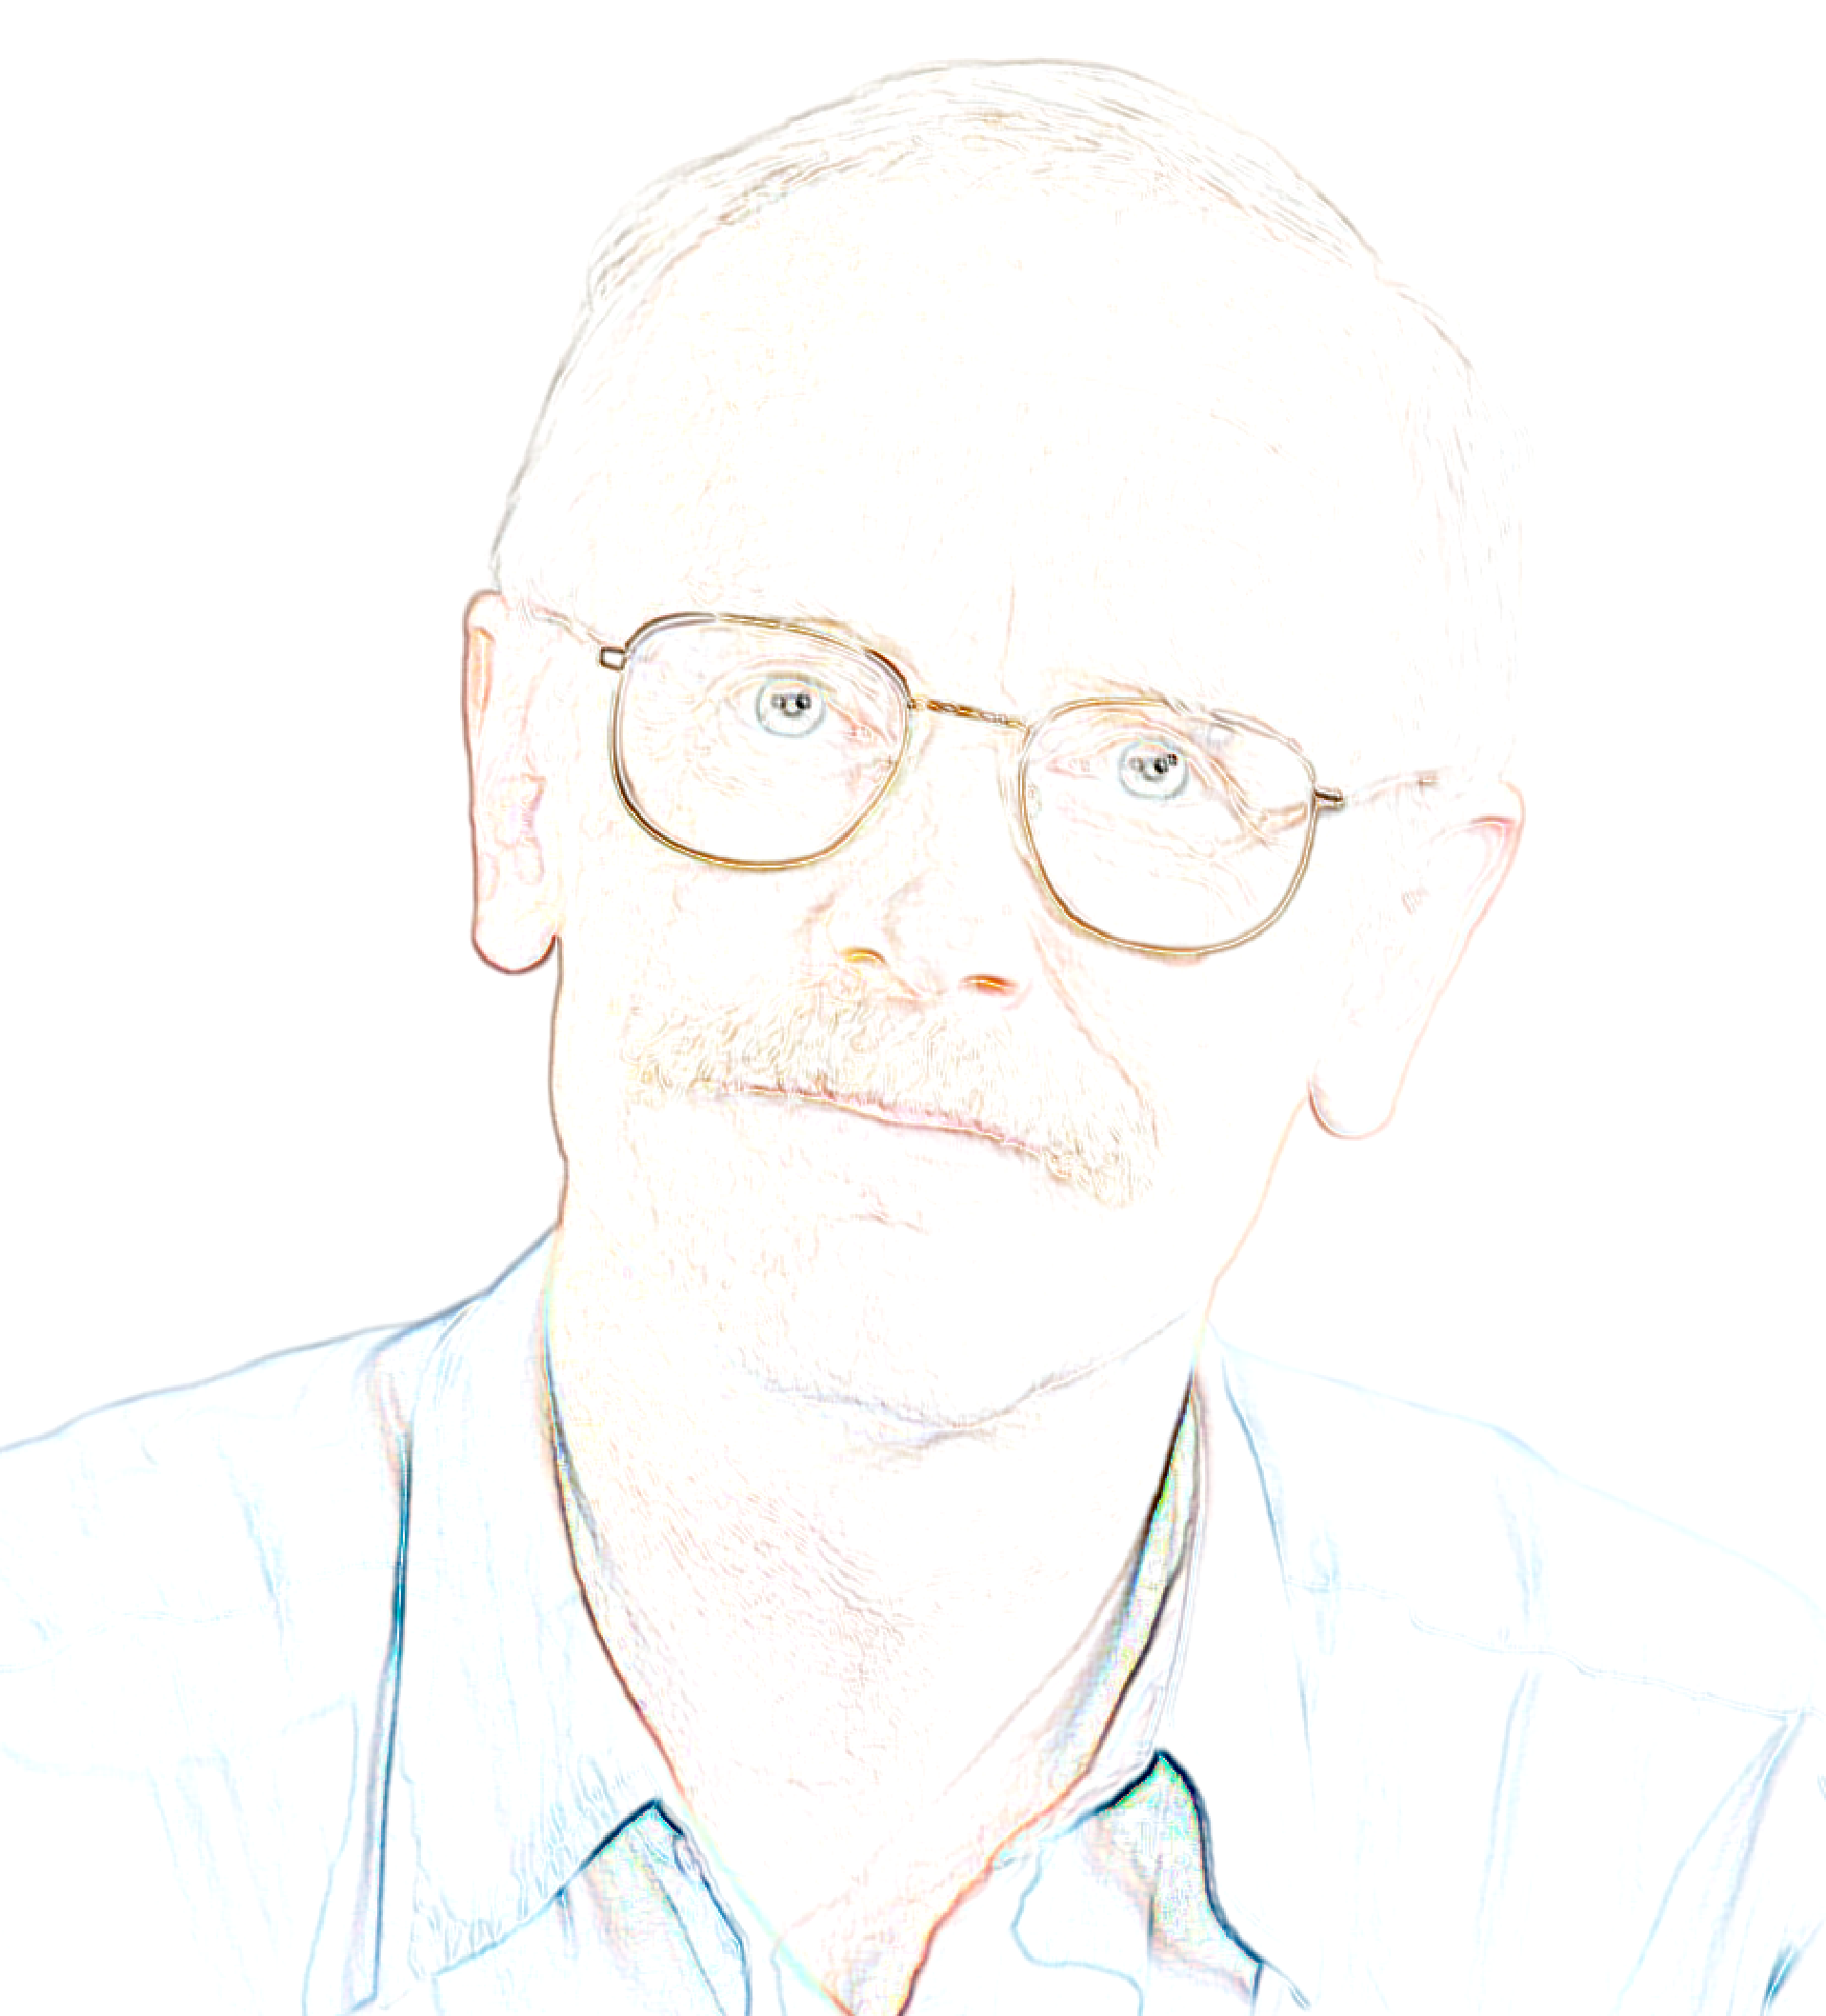
\includegraphics[width=0.618\columnwidth]{spacekg}
\caption[]{Gradients output for a real image}
\label{spacekq}
\end{figure}

\begin{figure}[ht!]
\centering

\includegraphics[width=0.618\columnwidth]{nsquare}
\caption[]{Noisy test square created with: \emph{paint 3}}
\label{nsquare}
\end{figure}

\begin{figure}[ht!]
\centering

\includegraphics[width=0.618\columnwidth]{nsquareg}
\caption[]{Gradients output for the noisy square}
\label{nsquareg}
\end{figure}

\begin{figure}[ht!]
\centering
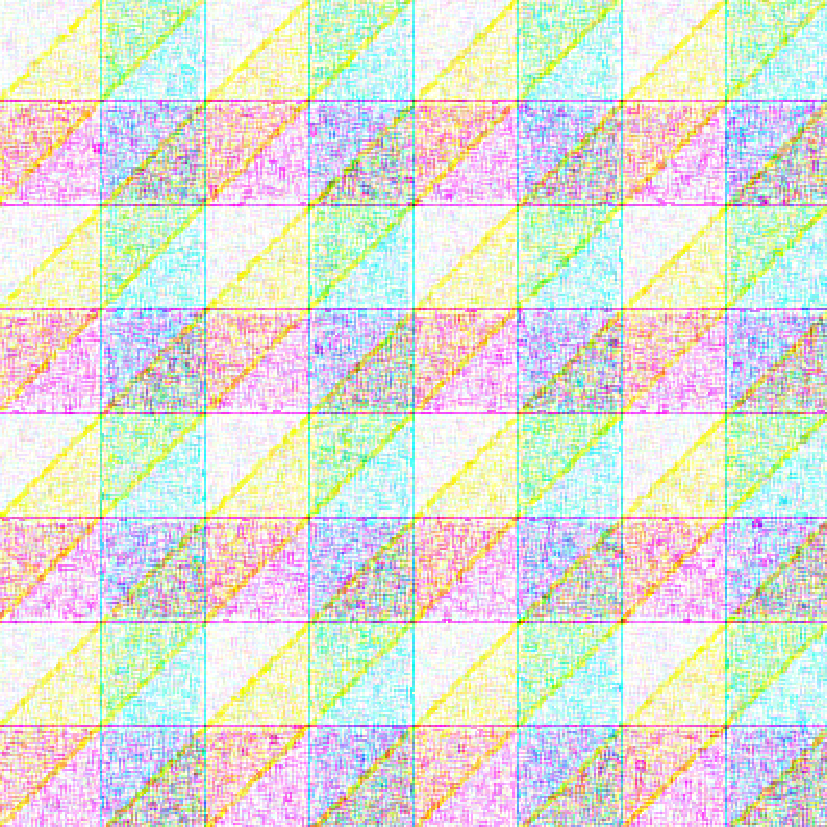
\includegraphics[width=0.618\columnwidth]{nsquaregm}
\caption[]{Noisy gradients field morphology: erosion and dilation}
\label{nsquaregm}
\end{figure}
\end{document}
